\documentclass[10pt,twoside=semi,openright,numbers=noenddot]{scrartcl}

\usepackage{amsmath,amssymb,amsthm}
\usepackage[usenames,svgnames,dvipsnames]{xcolor}
\usepackage{amsmath,amssymb,amsthm}
\usepackage{mathrsfs}
\usepackage[usenames,svgnames,dvipsnames]{xcolor}
\usepackage{hyperref}
\usepackage[nameinlink]{cleveref}
\usepackage{textcomp}
\usepackage{enumerate}
\usepackage{mathtools}
\usepackage{microtype}
\usepackage{geometry}
\usepackage[normalem]{ulem}
\usepackage{stmaryrd}
\usepackage{wasysym}
\usepackage{multirow}
\usepackage{prerex}
\usepackage{marginnote}
\usepackage{sidenotes}
\usepackage{mathtools}
\usepackage{epigraph}
\usepackage[headsepline ]{scrlayer-scrpage}
\usepackage[headsepline ]{scrlayer-scrpage}
\usepackage{thmtools}
\usepackage[framemethod=TikZ]{mdframed}
\usepackage{hyperref}
\usepackage[nameinlink]{cleveref}
\usepackage{setspace}
\usepackage{algorithm}
\usepackage{algpseudocode}
\usepackage{dirtytalk}
\usepackage[usenames,dvipsnames]{xcolor}
\definecolor{lightblue}{rgb}{0.68, 0.85, 0.9}
\definecolor{darkblue}{rgb}{0,0,0.5}
\renewcommand{\headfont}{}
\renewcommand*{\sectionmarkformat}{}



\newcommand{\SA}{\mathcal A}
\newcommand{\SB}{\mathcal B}
\newcommand{\SC}{\mathcal C}
\newcommand{\SD}{\mathcal D}
\newcommand{\SE}{\mathcal E}
\newcommand{\SF}{\mathcal F}
\newcommand{\SG}{\mathcal G}
\newcommand{\SH}{\mathcal H}
\newcommand{\SJ}{\mathcal J}
\newcommand{\SL}{\mathcal L}
\newcommand{\SM}{\mathcal M}
\newcommand{\cS}{\mathcal{S}}
\newcommand{\SP}{\mathcal P}
\newcommand{\SR}{\mathcal R}
\newcommand{\ST}{\mathcal T}
\newcommand{\SO}{\mathcal O}
\newcommand{\SX}{\mathcal X}
\newcommand{\SY}{\mathcal Y}

\newcommand{\iid}{\text{ i.i.d.}}


\renewcommand*{\marginfont}{\color{red}\sffamily}
\newcommand{\I}{\mathbb{}}

\newcommand{\II}{\mathbb I}
\newcommand{\CC}{\mathbb C}
\newcommand{\EE}{\mathbb E}
\newcommand{\FF}{\mathbb F}
\newcommand{\NN}{\mathbb N}
\newcommand{\QQ}{\mathbb Q}
\newcommand{\RR}{\mathbb R}
\newcommand{\mS}{\mathbb S}
\newcommand{\PP}{\mathbb P}
\newcommand{\VV}{\mathbb V}
\newcommand{\XX}{\mathbb X}
\newcommand{\YY}{\mathbb Y}
\newcommand{\ZZ}{\mathbb Z}



\newcommand{\eps}{\varepsilon}
\newcommand{\abs}[1]{\left\lvert #1 \right\rvert}
\newcommand{\norm}[1]{\left\lVert #1 \right\rVert}
\newcommand{\dang}{\measuredangle} %% Directed angle
\newcommand{\ray}[1]{\overrightarrow{#1}} 
\newcommand{\seg}[1]{\overline{#1}}
\newcommand{\arc}[1]{\wideparen{#1}}


\newcommand{\vocab}[1]{\textbf{\color{blue} #1}}
\newcommand{\term}[1]{\textit{\color{crimson} #1}}


\renewcommand*{\sectionformat}{\color{lava}\S\thesection\autodot\enskip}
\renewcommand*{\subsectionformat}{\color{Blue} \S\thesubsection\autodot\enskip}

\addtokomafont{partprefix}{\rmfamily}
\newcommand{\p}{\overset{p}{\to}}
\newcommand{\as}{\overset{a.s}{\to}}
\newcommand{\ds}{\overset{D}{\to}}
\newcommand*\note[1]{\begin{footnotesize}\begin{spacing}{1.0}\begin{fact}$\star$ #1\end{fact}\end{spacing}\end{footnotesize}}


%% round blue box
\theoremstyle{definition}
\mdfdefinestyle{mdbluebox}{%
	roundcorner = 10pt,
	linewidth=1pt,
	skipabove=12pt,
	innerbottommargin=9pt,
	skipbelow=2pt,
	nobreak=true,
	linecolor=blue,
	backgroundcolor=TealBlue!5,
	nobreak=true,
}
\declaretheoremstyle[
	headfont=\sffamily\bfseries\color{MidnightBlue},
	mdframed={style=mdbluebox},
	headpunct={\\[3pt]},
	postheadspace={0pt}
]{thmbluebox}


\mdfdefinestyle{mdbluebox*}{%
	skipabove=8pt,
	linewidth=1.5pt,
	rightline=false,
	leftline=true,
	topline=false,
	bottomline=false,
	linecolor=Blue!70!black,
	backgroundcolor=TealBlue!5,
	nobreak=true,
}
\declaretheoremstyle[
	headfont=\bfseries\sffamily\color{Blue!70!black},
	bodyfont=\normalfont,
	spaceabove=2pt,
	spacebelow=1pt,
	mdframed={style=mdbluebox*},
	headpunct={},
]{thmbluebox*}



\newenvironment{fact}{%
	\begin{mdframed}[linecolor=crimson!75,
	linewidth=1.5pt]}%
	{\end{mdframed}}
	
\mdfdefinestyle{baby-blue}{%
	linewidth=0.5pt,
	skipabove=12pt,
	frametitleaboveskip=5pt,
	frametitlebelowskip=0pt,
	skipbelow=2pt,
	frametitlefont=\bfseries,
	innertopmargin=4pt,
	innerbottommargin=8pt,
	nobreak=true,
	linecolor=light-blue!75,
	backgroundcolor=white,
}
\declaretheoremstyle[
	headfont=\bfseries\color{black},
	mdframed={style=baby-blue-box},
	headpunct={\\[3pt]},
	postheadspace={0pt},
]{baby-blue=box}



\mdfdefinestyle{mdblackbox-noline}{%
	skipabove=8pt,
	linewidth=1.5pt,
	rightline=false,
	leftline=false,
	topline=false,
	bottomline=false,
	linecolor=black,
	backgroundcolor=RedViolet!5!gray!5,
	nobreak=true,
}
\declaretheoremstyle[
	headfont=\bfseries,
	bodyfont=\normalfont,
	spaceabove=2pt,
	spacebelow=1pt,
	mdframed={style=mdblackbox-noline},
	headpunct={ --- }
]{thmblackbox-noline}
\definecolor{crimsonglory}{rgb}{0.75, 0.0, 0.2}
\definecolor{denim}{rgb}{0.08, 0.38, 0.74}
\definecolor{egyptianblue}{rgb}{0.06, 0.2, 0.65}
\definecolor{lava}{rgb}{0.81, 0.06, 0.13}


\definecolor{light-gray}{gray}{0.6}
\definecolor{lightlight-gray}{gray}{0.95}
\definecolor{light-blue}{RGB}{135,206,250}
\definecolor{crimson}{RGB}{220,20,60}
\definecolor{baby-blue}{RGB}{200,230,255}





\addtolength{\textheight}{3.14cm}
\setlength{\footskip}{0.5in}
\setlength{\headsep}{10pt}


\automark[subsection]{section}


\rohead{\footnotesize\thepage}
\rehead{\footnotesize \textbf{\sffamily Reinforcement Learning}, Hanan Ather}
% More script letters etc.


\hypersetup{
    colorlinks,
    linkcolor={red!50!black},
    citecolor={green!50!black},
    urlcolor={blue!80!black}
}


\mdfdefinestyle{mdbluebox**}{%
	linewidth=0.5pt,
	skipabove=12pt,
	frametitleaboveskip=5pt,
	frametitlebelowskip=0pt,
	skipbelow=2pt,
	frametitlefont=\bfseries,
	innertopmargin=4pt,
	innerbottommargin=8pt,
	nobreak=true,
	linecolor=Blue!70!black,
	backgroundcolor=TealBlue!5,
	nobreak=true,
}
\declaretheoremstyle[
	headfont=\bfseries\color{RawSienna},
	mdframed={style=mdredbox},
	headpunct={\\[3pt]},
	postheadspace={0pt},
]{thmredbox}




%% red boxes
%% red box square
\mdfdefinestyle{mdredbox}{%
	linewidth=0.5pt,
	skipabove=12pt,
	frametitleaboveskip=5pt,
	frametitlebelowskip=0pt,
	skipbelow=2pt,
	frametitlefont=\bfseries,
	innertopmargin=4pt,
	innerbottommargin=8pt,
	nobreak=true,
	linecolor=RawSienna,
	backgroundcolor=Salmon!5,
}
\declaretheoremstyle[
	headfont=\bfseries\color{RawSienna},
	mdframed={style=mdredbox},
	headpunct={\\[3pt]},
	postheadspace={0pt},
]{thmredbox}

%% red box line


\mdfdefinestyle{mdredbox}{%
	skipabove=8pt,
	linewidth=2pt,
	rightline=false,
	leftline=true,
	topline=false,
	bottomline=false,
	linecolor=RawSienna,
	backgroundcolor=Salmon!5,
}
\declaretheoremstyle[
	headfont=\bfseries\sffamily\color{RawSienna},
	bodyfont=\normalfont,
	spaceabove=2pt,
	spacebelow=1pt,
	mdframed={style=mdredbox*},
	headpunct={ --- },
]{thmredbox*}



\mdfdefinestyle{mdgreenbox}{%
	skipabove=8pt,
	linewidth=2pt,
	rightline=false,
	leftline=true,
	topline=false,
	bottomline=false,
	linecolor=ForestGreen,
	backgroundcolor=ForestGreen!5,
	nobreak=true,
}
\declaretheoremstyle[
	headfont=\bfseries\sffamily\color{ForestGreen!70!black},
	bodyfont=\normalfont,
	spaceabove=2pt,
	spacebelow=1pt,
	mdframed={style=mdgreenbox},
	headpunct={ --- },
]{thmgreenbox}
\declaretheoremstyle[
	headfont=\bfseries\sffamily\color{ForestGreen!70!black},
	bodyfont=\normalfont,
	spaceabove=2pt,
	spacebelow=1pt,
	mdframed={style=mdgreenbox},
	headpunct={},
]{thmgreenbox*}


%% New Green box
\mdfdefinestyle{mdgreenbox**}{%
	skipabove=8pt,
	linewidth=1pt,
	rightline=true,
	leftline=true,
	topline=true,
	bottomline=true,
	linecolor=ForestGreen,
	backgroundcolor=ForestGreen!5,
	nobreak=true
}
\declaretheoremstyle[
	headfont=\bfseries\sffamily\color{ForestGreen!70!black},
	bodyfont=\normalfont,
	spaceabove=2pt,
	spacebelow=1pt,
	mdframed={style=mdgreenbox**},
	headpunct={ --- },
]{thmgreenbox**}


\mdfdefinestyle{mdblackbox}{%
	skipabove=8pt,
	linewidth=1.5pt,
	rightline=false,
	leftline=true,
	topline=false,
	bottomline=false,
	linecolor=black,
	backgroundcolor=RedViolet!5!gray!5,
	nobreak=true,
}
\declaretheoremstyle[
	headfont=\bfseries,
	bodyfont=\normalfont,
	spaceabove=2pt,
	spacebelow=1pt,
	mdframed={style=mdblackbox},
	headpunct={ --- }
]{thmblackbox}






\declaretheorem[%
style=thmgreenbox**,name=Theorem,numberwithin=section]{theorem}
\declaretheorem[style=thmgreenbox,name=Lemma,sibling=theorem]{lemma}
\declaretheorem[style=thmbluebox,name=Corollary,sibling=theorem]{corollary}
\declaretheorem[name=Example,sibling=theorem]{example}
\declaretheorem[style=thmbluebox*,name=Definition,sibling=theorem]{definition}
\declaretheorem[name=Proposition,sibling=theorem]{proposition}

\newenvironment{moral}{%
	\begin{mdframed}[linecolor=green!70!black]%
	\bfseries\color{green!50!black}}%
	{\end{mdframed}}


\newenvironment{question}{%
	\begin{mdframed}[linecolor=red!70!black]%
	\bfseries\color{RawSienna}%
	\color{black} \textbf{Question:}} 
	{\end{mdframed}}


\declaretheoremstyle[
	headfont=\bfseries\color{RawSienna},
	mdframed={style=mdredbox},
	headpunct={\\[3pt]},
	postheadspace={0pt},
]{thmredbox}



\title{A Brief Overview of Reinforcement Learning}
\subtitle{MAT 5314 - Statistical Machine Learning}
\author{Hanan Ather}
\date{April 27, 2023}





\begin{document}
\maketitle
\tableofcontents
\newpage
\input{lectures/abstract}
\section{Introduction}
\subsection{What is Reinforcement Learning?}
Reinforcement Learning (RL) is a subfield of artificial intelligence that centers around an agent learning to make optimal decisions by interacting with its environment, receiving feedback in the form of rewards or penalties, and adjusting its behavior accordingly to maximize cumulative rewards over time \cite{RL}. In this process, the agent gathers information through actions and interactions with the environment, with its performance evaluated by the rewards it receives, which it ultimately aims to maximize.

Upon taking an action, the agent obtains two pieces of information: its present state within the environment and a real-valued reward \cite{RL2}. The agent's goal is to maximize its reward, thereby determining the most effective sequence of actions, or policy, to accomplish its objective. 
\begin{figure}
    \centering
    \tikzstyle{block} = [rectangle, draw, fill=blue!20,
    text width=8em, text centered, rounded corners, minimum height=4em]

    \tikzstyle{line} = [draw, -latex, color=blue]

    \begin{tikzpicture}[node distance = 6em, auto, thick]
        \node [block] (Agent) {\textbf{Agent}};
        \node [block, below of=Agent] (Environment) {\textbf{Environment}};
        
        \path [line] (Agent.0) --++ (4em,0em) |- node [near start]{Action $a_t$} (Environment.0);
        \path [line] (Environment.190) --++ (-6em,0em) |- node [near start] {New state  $s_{t+1}$} (Agent.170);
        \path [line] (Environment.170) --++ (-4.25em,0em) |- node [near start, right] {Reward $r_{t+1}$} (Agent.190);
    \end{tikzpicture}
    \caption{The MDP Framework: As illustrated in the figure, the agent, which represents an AI algorithm, and the environment, an abstract entity delivering uncertain outcomes, engage in a time-sequenced, iterative interaction. Credit: Adapted from Sutton \& Barto, 2018 \cite{RL} }
    \label{fig:my_label}
\end{figure}


\subsection{Supervised, Unsupervised, and Reinforcement Learning}
In contrast to supervised learning, where the learner trains passively using labeled data, reinforcement learning involves active engagement with the environment, and the policy chosen defines the distribution over observations rather than relying on a fixed distribution \cite{jordan2015}. Minor alterations to the policy can significantly impact the rewards obtained, highlighting the dynamic nature of reinforcement learning. Additionally, the environment may not remain constant and could change due to the actions selected by the agent \cite{buehler2019}. Reinforcement learning also differs from supervised learning in that training and testing phases are intertwined, rather than being separate stages of the process \cite{RL2}. 
Unlike other branches of machine learning, such as supervised and unsupervised learning, reinforcement learning embodies a more ambitious approach. It not only extracts patterns and properties from the given data, but also discerns suitable behaviors and decisions to progress towards the desired optimization objective \cite{RL}. One could argue that supervised and unsupervised learning primarily concentrate on ``minimization," as they strive to minimize the fitting error of a model to the provided data. Conversely, reinforcement learning focuses on ``maximization," seeking to identify the most appropriate decisions that contribute to the maximization of a well-defined objective.

In reinforcement learning, the agent confronts a dilemma between exploring unfamiliar states and actions to gather more information about the environment and rewards, and exploiting the existing information to optimize its reward. This challenge, known as the exploration versus exploitation trade-off \cite{RL2}, is a fundamental aspect of the reinforcement learning process.

\section{Basic Components of Reinforcement Learning}
\subsection{Markov Decision Process}
A Markov Decision Process (MDP) is a mathematical framework used in reinforcement learning to model decision-making in situations where an agent interacts with an environment that has probabilistic state transitions and rewards \cite{Markov}. 

The motivation for using MDPs in reinforcement learning is to provide a structured representation of the problem, facilitating the development of algorithms that enable agents to find optimal policies for maximizing cumulative rewards over time \cite{RL2}.
\begin{definition}[Markov Decision Process]
    MDP is defined by 4-tuple ($\cS$, $\SA$, $\SP_a$, $\SR$):
    \begin{enumerate}
        \item a set of states $\cS$, possibly infinite
        \item a set of actions $\SA$, possibly infinite
        \item  transition probability $\SP_a(s',s) = \PP [S_{t+1} = s'| S_{t} = ,A_{t} = a]$
        \item a reward $R_{t+1} \in \SR \subseteq \RR$, and corresponding probability distribution $ \SR_a(s',s) = \PP[r' | s,a]$ over rewards
    \end{enumerate}
\end{definition}

In a \textit{finite} MDP, random variables $R_t$ and $S_t$ possess well-defined discrete probability distributions, which depend solely on the preceding state and action. For specific values $r \in \SR$ and $s' \in \cS$, there exists a probability of these values occurring at time $t$, given particular values of the preceding state and action. The transition probabilities from one time step to the next can be represented as a function $\SP: \cS \times \SR \times 
\cS \times \SA \to [0,1]$, which is an ordinary deterministic function\cite{RL}:

\begin{equation}
    \SP(s', r \mid s, a) = \mathbb{P}\{S_{t+1} = s', R_{t+1} = r \mid S_t = s, A_t = a\}
\end{equation}
Markov Decision Processes (MDPs) have been used to model a wide range of decision-making problems across various domains, some read-world examples include:
\begin{itemize}
    \item Robotics: In robotics, MDPs are employed for navigation and path planning tasks \cite{thrun2005}
    \item Finance: MDPs have been used to model and solve portfolio optimization problems \cite{buehler2019}
    \item Healthcare: MDPs have been employed in healthcare for personalized treatment recommendation system 
    \cite{komorowski2018}
\end{itemize}

\subsection{Policy and Return}
In reinforcement learning algorithms, assessing the value of an agent being in a particular state is crucial. 
Almost all reinforcement learning algorithms involve estimates of how good is it for the agent to be in a given state \cite{RL}.
However, defining ``how good" a state is can be ambiguous. In RL, the value of a state is determined by anticipated future rewards, or more precisely, in terms of expected rewards.

Of course the rewards the agent can expect to receive in the future depends on the actions it will take. Accordingly, the values of states (i.e., the expected reward agent will receive from that state on wards) are defined with respect to a \vocab{policy}.

In reinforcement learning, a policy is a strategy or set of rules that guides an agent's decision-making process, determining which action to take in a given state to maximize cumulative rewards over time. Policies are just functions that take as input a state, $S_t$, and output a probability distribution of actions.
For a given state $s \in S$ and action $a \in A$, the policy is defined as \cite{mohri2018}:
\begin{definition}[Policy]
    A policy is a mapping $\pi: S \to \Delta(A),$ where $\Delta(A)$ is the set of probability distributions over the action space $A$. A policy is deterministic if for any $s \in S$, there exists a unique $a \in A$ such that $\pi(a|s) = 1$. In this case, we can identify $\pi: S \to A$.
    \footnote{The given definition pertains to a stationary policy, as the action distribution does not rely on time. Generally, a non-stationary policy can be characterized as a sequence of mappings $\pi_t : S \rightarrow \Delta(A)$, indexed by $t$. Notably, in scenarios with a finite horizon, employing a non-stationary policy is often essential for reward optimization}
\end{definition}
The objective in RL is to learn a policy, more precisely, the agent's objective is to find a policy that \textit{maximizes its expected (reward) return}. The discounted return is defined as \cite{RL}:
\begin{equation}
    G_t = R_{t+1} + \gamma R_{t+2 } + \gamma^2 R_{t+3 } + \cdots = \gamma^k \sum_{k=0}^{\infty} R_{t+k+1}
\end{equation}
Where $\gamma \in [0,1]$ is the \textit{discount-factor}\footnote{ The discount factor $\gamma$ serves to model scenarios in which a future reward is considered less desirable than an immediate reward of the same magnitude.}.
The return is a scalar-value that essentially summarizes a (possibly) infinite sequence of immediate rewards. 
An important fact to note is that even though this is an infinite sum, if $\gamma < 1$, $G_t$ will be finite, as long as $\{R_k\}$ is bounded \cite{RL}. If we set the value of $\gamma$ to $0$, the agent will only consider immediate reward, and future rewards will be of no consequence. Conversely, as  $\gamma \to 1$, the agent values future rewards more strongly \cite{RL}. The return $G_t$ for a given time step $t$ can be expressed recursively as:
\begin{align}
    G_t &= R_{t+1} + \gamma R_{t+2} + \gamma^2 R_{t+3} + \gamma^3 R_{t+4} + \cdots  \nonumber \\
    &= R_{t+1} + \gamma (R_{t+2} + \gamma R_{t+3} + \gamma^2 R_{t+4} + \cdots) \nonumber \\
    &= R_{t+1} + \gamma G_{t+1} \label{return}
\end{align}
By breaking down the computation of expected returns into smaller, incremental steps, the recursive property enables efficient updating of value estimates during the learning process. This is particularly useful in temporal difference learning methods, such as Q-learning and SARSA, where the value function is updated incrementally after each transition. This recursive property allows RL algorithms to leverage current estimates of future returns, $G_{t+1}$, to improve the current value estimate $G_t$. This process, known as bootstrapping, helps algorithms converge faster by taking advantage of information already available, rather than waiting to accumulate the complete return through the end of an episode. We will delve deeper into this idea in Section \ref{Algo}, where we explore Temporal Difference learning and Q-learning.

\subsection{Value and State-Value Functions}

Now we can define the notion of ``value of a state" formally via \vocab{value functions}. Value functions in RL are tools for estimating the long-term `value' or desirability of being in a given state. They allow the agent to access how good it is to be in a certain state, based on the expected cumulative reward obtained from that point onwards. There are two types of value functions commonly used in reinforcement learning: $V^{\pi}(s)$ and $Q^{\pi}(s,a)$, we define them formally below \cite{RL}, \cite{mohri2018}:
\begin{definition}[Value function]
    The value $V^{\pi}(s)$ for a fixed policy $\pi$ at a given state $s \in S$ represents the expected reward obtained when initiating at state $s$ and adhering to policy $\pi:$
    \begin{itemize}
        \item $V^{\pi}(s) = \underset{\pi, p}{\EE} [G_t \mid S_t = s]$for all $s \in S$ \cite{RL}
        \item finite horizon: $V^{\pi}(s) = \underset{a_t \sim \pi(s_t)}{\EE} \left[ \sum_{t=0}^T r(s_t,a_t) \mid S_t =s
        \right]$ \cite{mohri2018}
        \item infinite discounted horizon: $V^{\pi}(S_t = s) = \underset{a_t \sim \pi(s_t)}{\EE} \left[ \sum_{t=0}^{+ \infty} \gamma^t r(s_t,a_t) \mid S_t =s
        \right]$ \cite{mohri2018}     \footnote{Technically the notation should be: $\EE_{a_t \sim \pi(s_t)} \EE_{s_t}$ since
    we are not just taking the expectation over the random selection of an action $a_t$ according to the distribution $\pi(s_t)$, but we are also taking the expectation over the states $s_t$ reached and the corresponding reward values $r(s_t, a_t)$. However, in RL literature/textbooks the randomization with respect to the next state and reward function doesn't seem to be  explicitly mentioned (to simplify notation perhaps)} 
    \end{itemize}
\end{definition}
An intuitive way of understanding Value Function is that it tells us how much ``accumulated future reward'' we expect to obtain from a given state.

Starting from a state $s \in S$, to maximize reward, an agent naturally seeks a policy $\pi$ with the largest value $V_{\pi}(s)$. A remarkable result for finite MDPs in the finite horizon case, there exists an \textit{optimal policy} for all starting states $s \in S$. Formally, a policy $\pi^*$ is optimal if for any policy $\pi$ and any state $s \in S$, $V^{\pi^*}(s) \geq  V^{\pi}(s)$. 
We can prove that this optimal policy $\pi^*$ is deterministic \cite{mohri2018}, and this proof can be found in Mohri  et al. (2018). 
\\\
\\
\textbf{Action-Value Function} ($Q^{\pi}$): Represents the expected cumulative reward an agent can obtain by taking an action $a$ in a given state $s$ and following a certain policy $\pi$ thereafter. 

\begin{definition}[State-action value function]
    The state-action value function $Q$ associated to a policy $\pi$ is defined for all $(s,a) \in S \times A$ as the expected return for taking action $a \in A$ at state $s \in S$ and then following policy $\pi$:
    \begin{align*}
    Q^{\pi}(s,a) &=  \underset{\pi}{\EE} [G_t \mid S_t =s, A_t = a]  = \underset{\pi}{\EE}
    \left [
    \sum_{k =0}^{+ \infty} \gamma^t R_{t+k+1} \mid S_t = s, A_t = a \right ]
    \end{align*}
\end{definition}
The motivation behind using value functions in RL is to guide the agents decision-making process. By estimating the values of states or state-action pairs, the agent can choose actions that lead to states with higher-long term rewards. We will see in next section that values serve as the basis for various RL algorithms, such as $Q-$learning and SARSA.

Value functions $V^{\pi}$ and $Q^{\pi}$ can be estimated through experience. For instance, if an agent follows policy $\pi$ and maintains an average for each state encountered, based on the actual returns following that state, these averages will converge to $V^{\pi}(s)$ for all $s \in S$ as the number of times the state is encountered approaches infinity.
By keeping separate averages for each action taken in each state, these averages will converge to the action-values $Q^{\pi}(s,a)$. Such estimation methods are referred to as \textbf{Monte Carlo methods} because they involve averaging over numerous samples of actual returns.
\subsection{The Bellman Equations}
Value functions in reinforcement learning exhibit recursive relationships, like the one established for the return in equation (\ref{return}). For every policy $\pi$ and state $s$, this recursive relationship exists that links the value of $s$ to the values of its potential subsequent states \cite{RL}:
\begin{align*}
    V^{\pi}(s) &= \EE_{\pi}[G_t \mid S_t =s] \\
    &= \EE_{\pi}[R_{t+1} + \gamma G_{t+1} \mid S_t =s] \\
    &= \sum_{a \in A} \pi(a\mid s) \sum_{s'} \sum_{r} \PP(s',r \mid s,a) [r + \gamma \term{$\EE_{\pi} (G_{t+1} \mid S_{t+1} = s')$} ] \\
    &=\sum_{a \in A} \pi(a\mid s) \sum_{s'} \sum_{r} \PP(s',r \mid s,a) [r + \gamma \term{$V^{\pi}(s')$} ], \quad \forall s \in S
\end{align*}
The equation represents a recursive formulation of the value function, and this is known as the \vocab{Bellman Expectation Equation} \cite{RL}, \cite{RL2}, \cite{bellman1958}.
The Bellman equation is a fundamental equation in reinforcement learning and in dynamic programming. 
\note{In simple terms, the Bellman Equation decomposes the value function into immediate reward from taking an action in the current state plus the discounted expected value of future states, while taking into account all future possible actions.}
The Bellman equation tells us that the value of any state must be equal to the expected reward received from being in that state plus the (discounted) value of the expected next state.
Another more compact way to express the Bellman equation commonly found in the literature is: 
\begin{equation}\label{Bell1}
    V^{\pi}(s) = \sum_{a \in \SA(s)} \pi(a|s) \cdot \sum_{s'} \SP_{s,s'}^{a} [r(s,a) + \gamma V^{\pi}(s')]
\end{equation}
The equation states that the value of a given state, $V^{\pi}(s)$ under $\pi$, is equal to the immediate reward $r(s,a)$ plus discounted value of the next state $\gamma V^{\pi}(s')$. Recall that $V^{\pi}(s')$ is also an expectation, and therefore, it is considering all possible actions and transitions to the next state, weighted by their probabilities $\SP_{s,s'}^{a} = \PP(s' \mid s,a)$.
\\
Bellman Equation for Action-Value Function can be expressed in the same way:
\begin{align}
    Q^{\pi}(s,a) &= \SP_{s,s'}^{a} [ r(s,a) + \gamma \overbrace{\sum_{a'} \pi(a'|s') Q^{\pi}(s',a')}^{V^{\pi}(s)}] \\
    &= \SP_{s,s'}^{a} [ r(s,a) + \gamma V^{\pi}(s)]
\end{align}
Since, 
$$
V^{\pi}(s) = \sum_{a \in \SA(s)} \pi(a \mid s) Q^{\pi}(s,a)
$$
\subsection{Finding Optimal Policies}
Value functions allow us to create a hierarchical structure among policies, where a policy $\pi$ is deemed superior or equal to another policy $\pi'$ if it yields an expected return that is greater than or equal to that of $\pi'$ across all states \cite{RL2}. Thus, $\pi \geq \pi'$ if and only if the condition $V_\pi(s) \geq V_{\pi'}(s)$ holds true for every state $s \in S$ \cite{mohri2018}. For finite MDPs, there is always at least one policy that is better than or equal to all other policies \cite{RL}. This is what we call the \textit{optimal policy}. Although there might be more than one, we denote all the optimal policies by $\pi^*$. The optimal policies share the same state-value function and the action-value functions which we denote as $V^{*}$ and $Q^{*}$\cite{RL2}.
\begin{align*}
    V^{*}(s) = \underset{\pi}{\text{max }} V^{\pi}(s), \quad  \forall s \in S, a \in A \\ 
    Q^{*}(s) = \underset{\pi}{\text{max }} Q^{\pi}(s), \quad  \forall s \in S, \forall a \in A
\end{align*}
\note{
A useful fact which will be leveraging is that we can express $Q^*$ in terms of $V^*$:
\begin{align*}
    Q^*(s,a) &= \EE [R_{t+1} + \gamma V^*(S_{t+1}) \mid S_t = s, A_t =a ] \\ 
    &= \EE [R_{t+1}]  + \gamma \sum_{ s' \in \cS} \PP[S_{t+1} =s'|S_t = s, A_t = a] V^*(S_{t+1})   
\end{align*}
Note that $R_{t+1}$ is a random varible since we don't know what future state $s'$ we will end up in, therefore, 
we are taking the expectation $\EE [R_{t+1}]$ over the dynamics of transition probabilities of the next state $s'$ we reach.}
Recall that all value functions $v(s)$, must satisfy the recursive/self-consistency property established in (\ref{Bell1}). This mean we can express $V^*$ in a similar fashion. We write $V^*$ without  reference to any specific policy because it is the optimal value function. We follow a similar derivation which can be found in \cite{RL}, \cite{Markov}, \cite{RL2}, \cite{mohri2018}:
\begin{align}
    V^*(s) &= \underset{a \in A}{\text{max }} Q^{\pi}(s), \quad  \forall s \in S  \nonumber \\   
    &= \max_{a} \mathbb{E}_{\pi^*}[G_t \mid S_t = s, A_t = a] \nonumber \\
    &= \max_{a} \mathbb{E}_{\pi^*}[R_{t+1} + \gamma G_{t+1} \mid S_t = s, A_t = a] \nonumber \\
    &= \max_{a}  \mathbb{E}_{\pi^*}[R_{t+1} + \gamma V^*(S_{t+1}) \mid S_t = s, A_t = a] \nonumber \\
    &= \max_{a} \sum_{s'} \sum_{r} \PP(s',r \mid s,a) [r + \gamma V^{*}(s') ], \quad \forall s \in S 
\end{align}
This is known as the \vocab{Bellman Optimality Equation}. The equation expresses that ``the value of  state under \textit{optimal policy} must be equal to the expected for the best action from that state" \cite{RL}, and
is used to compute the optimal value function which is usually denoted as $V^*(s)$ in literature.
The Bellman optimally equation for $Q^*(s,a)$ is:
\begin{align*}
    Q^{*}(s,a) &= \EE \left [R_{t+1}
    + \gamma \underset{a}{\text{max}}Q^*(S_{t+1},a')  \mid S_{t} =s, A_t = a \right] \\
    &= \sum_{s',r}\PP(s',r \mid s,a)
    \left [r + \gamma \underset{a}{\text{max}}Q^*(S_{t+1},a') 
    \right]
\end{align*}
\textbf{Why are $Q^*$ and $V^*$ important?}
\begin{itemize}
    \item $V^*(s)$: When we have $V^*$, determining the optimal policy becomes easy. The beauty of $V^*$ lies in its ability to transform the greedy policy into the optimal policy in terms of long-term rewards \cite{RL}, as it takes into account the reward consequences of all possible future behaviors. Through $V^*$, the optimal expected long-term return is converted into a value that is readily and locally accessible for each state, allowing for more efficient decision-making \cite{RL}.
     
    \item $Q^*(s,a)$: With $Q^*$ at hand, the agent can bypass one-step ahead search. For any state $s \in S$, it can directly identify the action(s) that maximizes $Q^*(s,a)$. The action-value function serves as a cache for the results of one-step-ahead searches \cite{RL}, offering the expected long-term return as a value that is both locally and instantly accessible for each state-action pair.
\end{itemize}




\section{Reinforcement Learning Algorithms}\label{Algo}
Thus far we have been under the assumption that we have access to a model of the Markov Decision Process (MDP) environment, which includes transition states defined by $\mathcal{S}$ and the probabilities of the next state and reward given the current state and action\footnote{By model we mean the transition states define by $\SP$, probabilities of next state and reward, given current state and reward}.
However, in real-world scenarios, we often lack access to an MDP model. 
When we don't have a model, we don't have access to the environment's dynamics such as transition probabilities, $\PP(S_{t+1} \mid S_t , A_t)$, or rewards functions $r(s_{t+1}, a_t, s_t)$ . Consequently, we cannot predict the next state and the immediate reward you will receive when taking a specific action in a given state. 
Instead, the agent must interact with the actual MDP environment to learn about it. Interacting with the environment doesn't provide transition probabilities; it simply presents a new state and reward when an action is taken in a specific state. The environment supplies individual experiences of the next state and reward, rather than the explicit probabilities of occurrence for the next states and rewards. This raises a pertinent question: is it possible to compute the optimal value function or optimal policy without access to a model?

\subsection{Model-based and Model-free learning}
In RL literature, there are primarily two approaches:  Model-based and Model-free learning \cite{RL3}. In model-based learning approaches, the agent first learn a model of the environment before proceeding to learn a policy \cite{RL2}. In this approach, the agent creates an internal model of the environment, including its rules and dynamics. Once this model is established, the agent then uses it as a guide to learn and refine an  policy. This approach can be more computationally demanding, but it often leads to a more robust and flexible policy, because the agent can use its understanding of the environment to plan and adapt its actions to different situations \cite{RL}.
Model-free approach, involves directly acquiring an action policy without necessarily understanding the underlying dynamics of the environment. The learning agent learns the environment based on the rewards it receives, without developing a comprehensive understanding of how the environment actually works \cite{RL3}. The Q-learning algorithm  discussed in the next section belongs to the group of model-free methods.



\subsection{On-policy and Off-Policy Methods}
The distinction between ``on-policy" and ``off-policy" methods lies in the relationship between the policy that the agent follows while exploring the environment (behaviour policy) and the policy that it learns about (target policy). 

\begin{itemize}
    \item \textbf{On-policy methods:} 
    These are the methods where the policy that's being improved upon is the same policy that's used to make decisions during interaction with the environment. In other words, the agent learns about and improves the policy that it is currently following. SARSA is a common example of an on policy method.
\end{itemize}
 

\subsection{Temporal difference learning}

The Temporal-Difference (TD) learning method is prevalently employed in reinforcement learning applications \cite{RL3}.. TD learning is a method for estimating the expected cumulative future reward, or ``value," of each state in an environment. This value is updated at each time increment based on the difference between the predicted value of a state and the observed value after taking an action and transitioning to a new state \cite{RL}, \cite{RL2}.
TD learning leverages a hybrid approach that combines Monte Carlo's model-free experience-based value estimation with the benefits of dynamic programming's capability to calculate values utilizing present estimates alone \cite{sutton1988b}. 
\begin{equation}
    V(S_t) \leftarrow V(S_t) + \alpha(R_{t+1} + \gamma \cdot V(S_{t+1} - V(S_t))
\end{equation}
\begin{itemize}
    \item We refer to $R_{t+1} + \gamma \cdot V(S_{t+1})$ as the \textbf{TD target}
    \item We refer to $\delta_{t} = R_{t+1} + \gamma \cdot V(S_{t+1}) - V(S_{t})$ as  \textbf{TD error}
\end{itemize}
The TD target is a (biased) estimate of $G_t$ \cite{RL}. The TD control algorithm can update the Q-value function after each time step. 



\subsection{Q-learning}
One of the most well-known and widely used model-free RL methods is Q-learning, which was proposed by proposed by Watkins (1989) \cite{watkins1989}, and has been instrumental in solving various decision-making problems. One of the most renowned applications of Q-learning is in the use of a more advanced version called Double Q-learning, a modification of the Deep Q-Network (DQN). This method was employed to train agents to play 49 games on the Atari 2600 system \cite{van2016double}.
Q-learning is a specific implementation of TD learning that seeks to learn the value of taking a particular action in a particular state, also known as the Q-value \cite{RL}. These Q-values are stored in a table and updated using a similar temporal difference method. The Q-learning algorithm is model-free, meaning it doesn't require knowledge of the underlying environment model. Instead, it learns from direct interaction with the environment.
The goal of the Q-learning algorithm is to seek Q-function (our case table of state-action pairs) which represents the expected cumulative reward for taking a particular action in a given state and following the optimal policy thereafter. The agent starts with an initial Q-table and iteratively updates its Q-values based on the observed reward and the next state values.
The update rule for Q-learning is given by \cite{watkins1992}:
\begin{equation}
    Q(S_t,A_t) \leftarrow
    Q(S_t,A_t) + \alpha
    \left [
    R_{t+1} + \gamma \underset{a}{\text{max}}
    Q(S_{t+1},a) - Q(S_t, A_t)
    \right]
\end{equation}
Its important to note that the optimal policy ($\pi^*$) or optimal value function ($V^*$) can be directly obtain from $Q*$ by the following computations: $\pi^*(s) = \underset{a \in \SA}{\text{argmax }} Q^*(s,a)$ and $V^*(s) = \underset{a \in \SA}{\text{max }} Q^*(s,a)$.

\begin{algorithm}
\caption{Q-learning Algorithm}\label{Q-learning}
\begin{algorithmic}
\Require a step size  $\alpha \in [0,1]$, and $\epsilon \in [0,1]$ ($\epsilon$ is generally chosen to be a very small value)
\Ensure $Q(s,a)$ for all $s \in \cS, a \in \SA(s)$ is initialized
\For {each episode}
\State Initialize $S$
\For {each step of episode:} 
    \State Choose action $a \in \SA(s)$, given state $s \in \cS$, using policy $\pi$ derived from $Q(s,a)$ 
    \State ($\epsilon-$ greedy)
    \State Take action  $a$, and observe $r$ and $s'$
    \State $Q(s,a) \leftarrow
    Q(s,a) + \alpha
    \left [
    r + \gamma \underset{a'}{\text{max}}
    Q(s',a') - Q(s, a)
    \right]$
    \State \textbf{Update State:} $s \leftarrow s'$
    \EndFor \Comment{Until $s$ is terminal state} \\
    \textbf{Return:} $Q$ table 
\end{algorithmic}
\end{algorithm}
The pseudo code above adapted from Sutton \& Barto (2018) \cite{RL} and Mohri et al. (2018) \cite{mohri2018}.
Note that we are taking advantage of the recursive structure of the Value Function as given by the Bellman Equation; we only have access to individual experiences of next state $S_{t+1}$ and reward $R_{t+1}$, and not the transition probabilities of next state and  reward, and we are approximating $G_t$ by $R_{t+1} + \gamma V(S_{t+1})$. 
In recent years, due to the rise of deep neural networks, Q-learning has been successfully applied in a diverse set of domains, showcasing its versatility and adaptability. 

\section{Results}
\subsection{Simulation: GridWorld}

Gridworld is a commonly used environment in the study of reinforcement learning \cite{RL}. Our version of GridWorld is set up as a simple maze, where the agent needs to find the quickest route to the exit.
It is typically represented as a two-dimensional matrix, where each cell in the grid corresponds to a different state that an agent could be in. We used GirdWorld as a toy environment to learn an optimal policy via Q-learning.

Our agent begins at the most top left corner cell, and learns moving from one cell to another, in order to reach the final cell at the bottom right corner. The agent can choose from 4 actions: up, down, left, or right.

States or cells in the grid  have different properties. All cells excepts the final cell at the bottom right corner give the agent a reward of -1, the final cell (end state) give the agent a reward of +1. This reward structure forces  the agent  to find the quickest route to the exit.

Our implementation of GirdWorld takes in 5 user-defined hyper parameters, can be easily modified at the begin of the program. Different hyperparameters in the Q-learning algorithm can impact the agent's learning performance and overall behavior. Here's an overview of the hyperparameters and how they can influence the agent based on our experiments and literature:
\begin{enumerate}[(i)]
    \item \textbf{Learning rate} $\alpha$: This parameter determines how much the agent updates its Q-values based on new information. A high learning rate means the agent gives more importance to recent experiences, while a low learning rate indicated it relies more on its accumulated knowledge. We found if the learning rate was set too high, the agent sometimes failed to converge or learned a suboptimal policy. If it's set too low, the ``learning process"  was slow or the agent may get stuck in a local optimum .

    \item \textbf{Discount factor} $\gamma$: As discussed earlier, this parameter determines how much the agent values future rewards compared to immediate rewards. High discount factor means the agent puts more emphasis on long-term rewards, while a low discount factor makes the agent more focused on short-term rewards. If the discount factor is too high, the agent may take longer to learn an optimal policy, as it needs to explore more steps into the future. If it's too low, the agent may learn a suboptimal policy that only focuses on short-term gains.
    
    \item \textbf{Initial Exploration rate} $\epsilon$: This parameter determines the initial probability that the agent chooses a random action instead of the action with the highest Q-value \cite{RL}. A high exploration rate means the agent explores the environment more, while a low exploration rate means the agent focuses more on exploiting its current knowledge. If the exploration rate is too high, the agent took longer to learn an optimal policy, as it spends more time exploring. If it is set too low, the agent may not explore enough to find the best actions and learn a suboptimal policy.

    \item \textbf{Exploration Decay rate}: This parameter determines how fast the exploration rate decreases over time. A high decay rate means the agent reduces its exploration rate quickly, while a low decay rate means the agent maintains a higher exploration rate for longer. We found if the decay rate is too high, the agent may not explore enough to learn an optimal policy. If it was set too low, the agent took longer to converge, as it continued to explore even when it has already learned a good policy.

    \item \textbf{Number of raining episodes} $n$ : This parameter sets the total number of episodes the agent goes through. We found if we set the number of episodes too low, the agent may not have enough time to learn an optimal policy. And if we set it too high, the agent wasted computational resources without significant improvements in performance.

\end{enumerate} 
Tuning these hyperparameters essentially comes down to finding a balance between exploration and exploitation, learning speed and stability, and short-term and long-term rewards. We can use techniques like grid search, random search, or Bayesian optimization to find the optimal combination of hyperparameters for this specific problem, however, exploration of this will be outside the scope of this paper.

\begin{figure}\label{result}
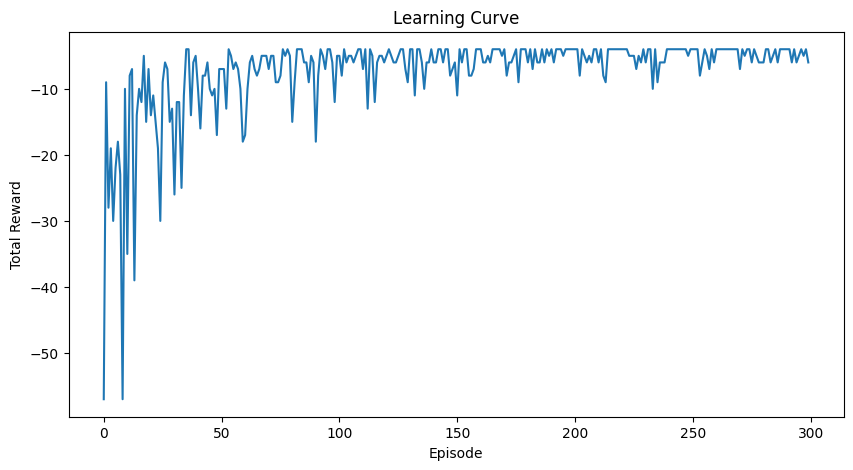
\includegraphics[width=12cm]{lectures/diagrams/result.png}
\centering
\caption{Result from simulation of GridWorld}
\end{figure}
\subsection{Conclusion}
We conclude our discussion with a Figure (2) that provides concrete evidence that our agent is indeed capable of learning a policy that exhibits improvement over successive episodes. As can be clearly observed in the graph, there is a notable increase in the total reward, on average, as the number of episodes escalates. This trend of increasing total reward signifies the agent's progressive learning and adaptation.

The occasional downward spikes in the graph represent instances where the agent chooses to take ``exploratory" actions as opposed to the optimal or ``greedy" action. This is a crucial part of the learning process, allowing the agent to explore a broader range of possible actions and outcomes, thus avoiding the potential pitfall of premature convergence on a suboptimal policy.

Over time, it is observable that the probability of these ``exploratory" actions diminishes, which is indicative of the agent settling into an optimal policy. As a consequence, the total return exhibits greater stability, with fluctuations becoming increasingly infrequent and minor. This illustrates the agent's successful adaptation and the maturing of its learned policy, reinforcing the validity of our approach.


 

\phantomsection
\begin{thebibliography}{99}


\bibitem{RL}Sutton, Richard S and Barto, Andrew G \textit{Reinforcement learning: An introduction}. MIT press, 2018.

\bibitem{jordan2015}Jordan, M.I. and Mitchell, T.M. \textit{Machine learning: Trends, perspectives, and prospects}. Science, 349(6245):255--260, 2015.

\bibitem{Markov}Puterman, Martin L \textit{Markov Decision Processes: Discrete Stochastic Dynamic Programming}. John Wiley \& Sons, Inc., 1994.

\bibitem{RL2}Russell, Stuart J and Norvig, Peter \textit{Artificial intelligence: a modern approach}. MIT press, 2016.


\bibitem{thrun2005}Thrun, Sebastian and Burgard, Wolfram and Fox, Dieter \textit{Probabilistic Robotics}. MIT Press, 2005. \url{https://docs.ufpr.br/~danielsantos/ProbabilisticRobotics.pdf}


\bibitem{komorowski2018}Komorowski, Matthieu and Celi, Leo Anthony and Badawi, Omar and Gordon, Anthony C. and Faisal, A. Aldo \textit{The Artificial Intelligence Clinician learns optimal treatment strategies for sepsis in intensive care}. Nature Medicine, 24:1716–1720, 2018. \url{https://finale.seas.harvard.edu/publications/guidelines-reinforcement-learning-healthcare}



\bibitem{buehler2019}Buehler, Stefan and Ranganathan, Arun and Gupta, Rahul \textit{Reinforcement Learning for Finance}. Stanford University, 2019. \url{https://stanford.edu/~ashlearn/RLForFinanceBook/book.pdf}


\bibitem{mohri2018}Mohri, Mehryar and Rostamizadeh, Afshin and Talwalkar, Ameet \textit{Foundations of Machine Learning}. The MIT Press, 2018. \url{https://cs.nyu.edu/~mohri/mlbook/}


\bibitem{bellman1958}Bellman, Richard \textit{Dynamic Programming and Stochastic Control Processes}. Information and Control, 1:228--239, 1958.

\bibitem{sutton1988b}Sutton, Richard S. \textit{Learning to Predict by the Methods of Temporal Difference}. Machine Learning, 3:9--44, 1988.

\bibitem{watkins1989}Watkins, Christopher JCH. \textit{Learning from Delayed Rewards}. PhD Thesis, University of Cambridge, England, 1989.





\bibitem{watkins1992}Watkins, Christopher JCH and Dayan, Peter \textit{Q-learning}. Machine Learning, 8(3):279--292, 1992.




\bibitem{bdr2022}Marc G. Bellemare and Will Dabney and Mark Rowland \textit{Distributional Reinforcement Learning}. MIT Press, 2023.


\bibitem{Goodfellow-et-al-2016}Ian Goodfellow and Yoshua Bengio and Aaron Courville \textit{Deep Learning}. MIT Press, 2016. \url{http://www.deeplearningbook.org}

\bibitem{RL3}Dimitri Bertsekas \textit{Reinforcement Learning and Optimal Control}. MIT Press, 2019.



\bibitem{kober2013}Kober, Jens and Bagnell, J. Andrew and Peters, Jan \textit{Reinforcement Learning in Robotics: A Survey}. International Journal of Robotics Research, 2013. \url{https://www.ri.cmu.edu/pub_files/2013/7/Kober_IJRR_2013.pdf}

\bibitem{van2016double}Van Hasselt, Hado and Guez, Arthur and Silver, David \textit{Deep Reinforcement Learning with Double Q-learning}. Proceedings of the Thirtieth AAAI Conference on Artificial Intelligence, 2016. \url{https://www.davidsilver.uk/wp-content/uploads/2020/03/doubledqn-1.pdf}




\end{thebibliography}
\end{document}
